\begin{frame}
  \frametitle{Benchmark}
  \framesubtitle{Average Results}
  \monocolumn{
    \scalebox{0.9}{
      \begin{tikzbenchmarkfig}

        \begin{pgfonlayer}{background}
          \node[main plot](main){%
            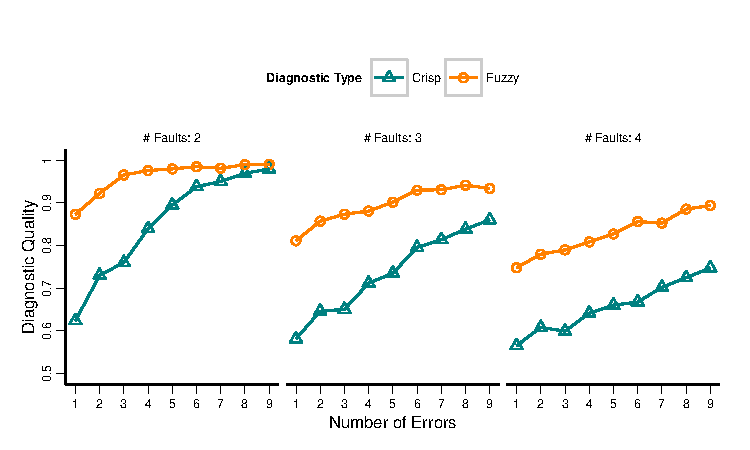
\includegraphics[trim=1.15cm 1.15cm 0.5cm 2.5cm,clip]{figures/fuzzinel/plot2.pdf}%
          };
        \end{pgfonlayer}
        \node[below=0cm of main.south] (axisx){
          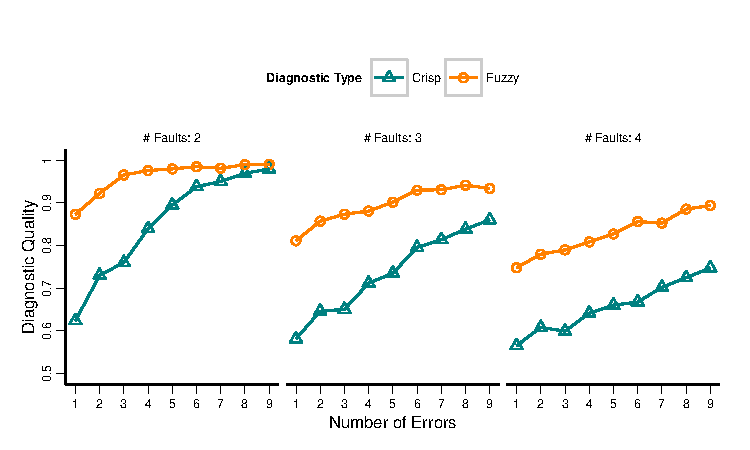
\includegraphics[trim=1.15cm 0.7cm 0.5cm 6.55cm,clip]
          {figures/fuzzinel/plot2.pdf}};
        \node[below=0.1cm of axisx.south ]{$\#$ of Errors};
        \node[left=0cm of main.north west, anchor=north east] (axisy){
          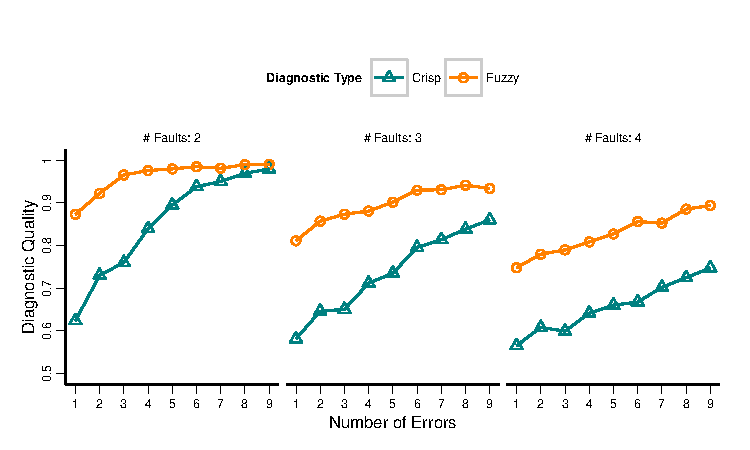
\includegraphics[trim=0.7cm 1.15cm 11.6cm 2.5cm,clip]
          {figures/fuzzinel/plot2.pdf}};
        \node[anchor=east,left=0.1cm of axisy.west] {
          \rotatebox{90}{Diagnostic Quality}};

        \node[above=0.5cm of main.north, anchor=south] (capt){
          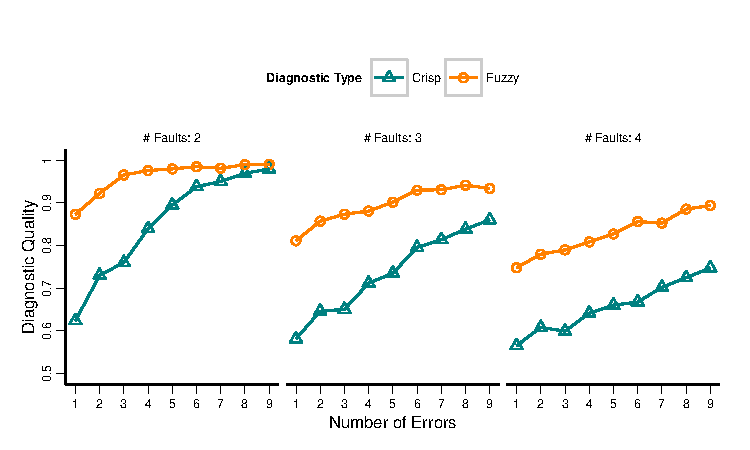
\includegraphics[trim=1.15cm 5cm 0.5cm 1cm,clip]
          {figures/fuzzinel/plot2.pdf}};
      \end{tikzbenchmarkfig}
    }
  }
  \note{
    \begin{itemize}
    \item explicar setup
    \item Fuzzinel conseguiu tirar proveito da info dos sintomas de
      erro para melhorar a qualidade de diagnostico
    \end{itemize}
  }
\end{frame}
